\pgfplotsset{
    width=\textwidth*0.5,
    tick label style={font=\footnotesize},
    label style={font=\small},
    legend style={font=\tiny},
}

% Example of a figure that spans the whole page width and with subfigures. The same concept works for tables, too.
\begin{figure}[htb]
%\isPreprints{}{% This command is only used for ``preprints''.
%\begin{adjustwidth}{-\extralength}{0cm}
\centering
%} % If the paper is ``preprints'', please uncomment this parenthesis.
\subfloat[\centering]{
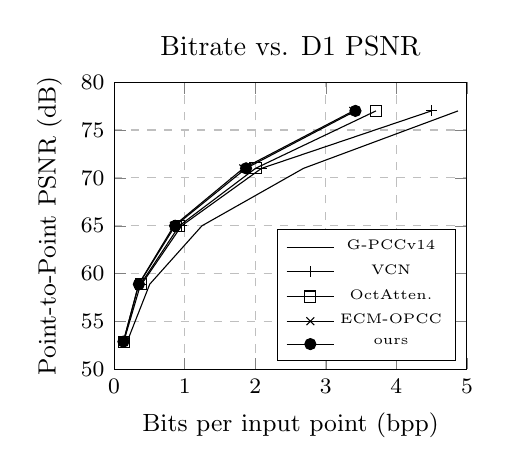
\begin{tikzpicture}
\begin{axis}[
    title={Bitrate vs. D1 PSNR},
    xlabel={Bits per input point (bpp)},
    ylabel={Point-to-Point PSNR (dB)},
    xmin=0, xmax=5,
    ymin=50, ymax=80,
    xtick={0,1,2,3,4,5},
    ytick={50,55,60,65,70,75,80},
    legend pos=south east,
    xmajorgrids=true,
    ymajorgrids=true,
    grid style=dashed,
]

\addplot[
    color=black
]
coordinates {
    (0.185,52.9)(0.505,58.9)(1.245,65.0)(2.684,71.0)(4.874,77.0)
};
\addlegendentry{G-PCCv14}

\addplot[
    color=black,
    mark=+,
]
coordinates {
   (0.390,58.9)(0.956,65.0)(2.089,71.0)(4.497,77.0)
};
\addlegendentry{VCN}

\addplot[
    color=black,
    mark=square,
]
coordinates {
    (0.137,52.9)(0.376,58.9)(0.924,65.0)(2.004,71.0)(3.711,77.0)
};
\addlegendentry{OctAtten.}

\addplot[
    color=black,
    mark=x,
]
coordinates {
    (0.131,52.9)(0.348,58.9)(0.847,65.0)(1.831,71.0)(3.39,77.0)
};
\addlegendentry{ECM-OPCC}

\addplot[
    color=black,
    mark=*,
]
coordinates {
    (0.132,52.9)(0.351,58.9)(0.865,65.0)(1.87,71.0)(3.42,77.0)
};
\addlegendentry{ours}
    
\end{axis}
\end{tikzpicture}
}
\hfill
\subfloat[\centering]{
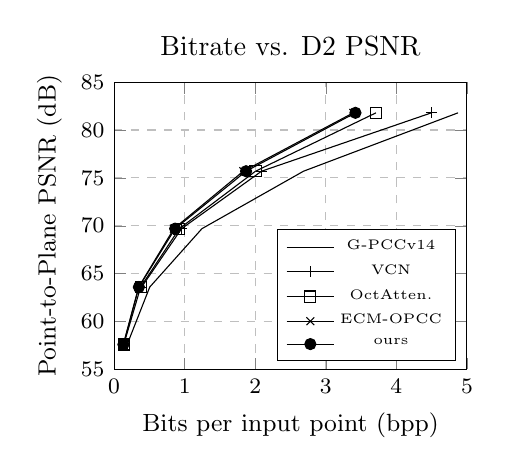
\begin{tikzpicture}
\begin{axis}[
    title={Bitrate vs. D2 PSNR},
    xlabel={Bits per input point (bpp)},
    ylabel={Point-to-Plane PSNR (dB)},
    xmin=0, xmax=5,
    ymin=55, ymax=85,
    xtick={0,1,2,3,4,5},
    ytick={55,60,65,70,75,80,85},
    legend pos=south east,
    xmajorgrids=true,
    ymajorgrids=true,
    grid style=dashed,
]

\addplot[
    color=black
]
coordinates {
    (0.185,57.6)(0.505,63.6)(1.245,69.7)(2.684,75.7)(4.874,81.8)
};
\addlegendentry{G-PCCv14}

\addplot[
    color=black,
    mark=+,
]
coordinates {
   (0.390,63.6)(0.956,69.7)(2.089,75.7)(4.497,81.8)
};
\addlegendentry{VCN}

\addplot[
    color=black,
    mark=square,
]
coordinates {
    (0.137,57.6)(0.376,63.6)(0.924,69.7)(2.004,75.7)(3.711,81.8)
};
\addlegendentry{OctAtten.}

\addplot[
    color=black,
    mark=x,
]
coordinates {
    (0.131,57.6)(0.348,63.6)(0.847,69.7)(1.831,75.7)(3.39,81.8)
};
\addlegendentry{ECM-OPCC}

\addplot[
    color=black,
    mark=*,
]
coordinates {
    (0.132,57.6)(0.351,63.6)(0.865,69.7)(1.87,75.7)(3.42,81.8)
};
\addlegendentry{ours}
    
\end{axis}
\end{tikzpicture}
}
%\isPreprints{}{% This command is only used for ``preprints''.
%\end{adjustwidth}
%} % If the paper is ``preprints'', please uncomment this parenthesis.
\caption{
Results of our proposed MIC-OPCC model against state-of-the-art baselines on the SemanticKITTI dataset. While achieving comparable compression ratios to OctAttention, our model significantly outperforms it in both encoding and decoding speed.
\label{fig:kitti_plot}
}
\end{figure} 